\documentclass[tikz,border=10pt]{standalone}
\usepackage{pgfplots}
\pgfplotsset{compat=1.18}
\usetikzlibrary{arrows.meta}

\begin{document}
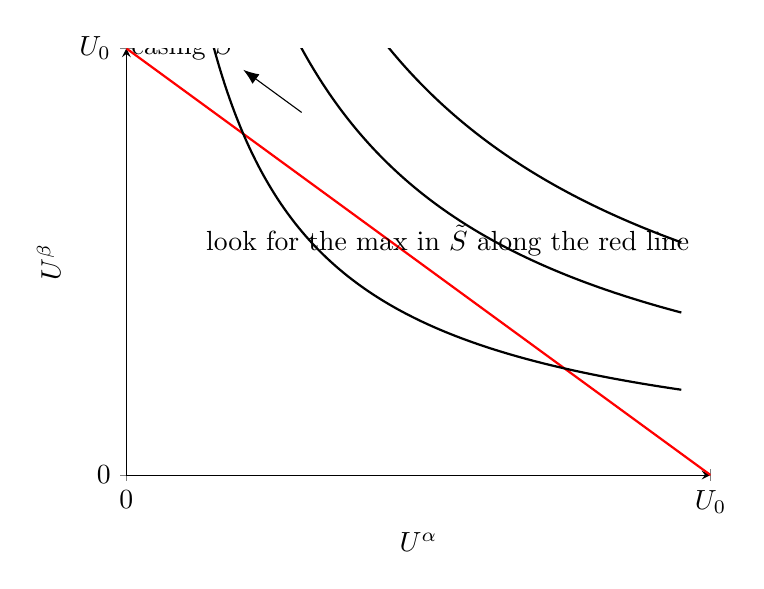
\begin{tikzpicture}
\begin{axis}[
    width=9cm,
    height=7cm,
    xmin=0, xmax=1,
    ymin=0, ymax=1,
    xlabel={$U^\alpha$},
    ylabel={$U^\beta$},
    axis lines=left,
    xtick={0,1},
    ytick={0,1},
    xticklabels={$0$,$U_0$},
    yticklabels={$0$,$U_0$}
]
    % Constraint line U^alpha + U^beta = U0
    \addplot[red,thick] coordinates {(0,1) (1,0)};

    % Contour-like curves (level sets)
    \addplot[black,thick,domain=0.05:0.95,samples=200] {0.2/(x+0.05)};
    \addplot[black,thick,domain=0.1:0.95,samples=200] {0.4/(x+0.1)};
    \addplot[black,thick,domain=0.2:0.95,samples=200] {0.6/(x+0.15)};

    \node at (axis cs:0.55,0.55) {look for the max in $\tilde{S}$ along the red line};
    \draw[-{Latex[length=2mm]}] (axis cs:0.3,0.85) -- (axis cs:0.2,0.95) node[above left] {increasing $\tilde{S}$};
\end{axis}
\end{tikzpicture}
\end{document}
